\section{Технический проект}

\subsection{Общие сведения о программной системе}
Необходимо спроектировать и разработать распределенную систему для поиска информации по документам из Интернет-пространства.

Системе на вход подается некоторое множество адресов WEB-ресурсов.
Предполагается, что пространство документов связное и что через данное множество ресурсов достижимы все остальные документы целевого графа, чтобы система в перспективе своей работы могла бы целиком обработать пространство документов, которое соответствует начальному множеству.

Ключевыми компонентами системы будут являться:
\begin{itemize}
\item поисковый робот;
\item индексатор;
\item поисковик;
\item сборщик журналируемой информации.
\end{itemize}

Компоненты имеют кардинально разные требования по функциональности и режимам работы, поэтому должны быть спроектированы независимо друг от друга для достижения низкой связанности и возможности горизонтального масштабирования системы.

Целью разработки данной распределенной программной системы является создание инструмента для эффективного ориентирования в таком быстрорастущем сегменте хранения информации как Интернет.

\subsection{Обоснование выбора технологий проектирования}
Используемые для создания программно-информационной системы
языки и технологии отвечают современным практикам разработки, позволяют достичь высокой производительности и отказоустойчивости системы.

\subsubsection{Язык программирования C++}

Язык программирования C++ является мультипарадигменным компилируемым языком со статической типизацией. Его основные преимущества заключаются в высокой производительности, гибкости, тесной связи с аппаратным обеспечением и поддержкой самых разнообразных конструкций из ООП. Эффективность всех компонентов системы будет зависеть от степени задержки выполняемых операций, поэтому С++ можно считать оптимально подходящим под запросы разработки.

\subsubsection{CMake}

CMake - это кроссплатформенная утилита, автоматизирующая процесс создания файлов сборки для таких компилируемых языков, как C++. В частности, в ОС GNU Linux она генерирует Makefile, который, как известно, ответственен за сборку всех имеющихся исходных файлов в один исполняемый. 

\subsubsection{Vcpkg}
Vcpkg -- кроссплатформенный пакетный менеджер с открытым исходным кодом, созданный Microsoft. Призван упростить интеграцию сторонних библиотек на языках C и C++ c учетом архитектуры процессора и операционной системы устройства. Очень полезен в случае, когда проект использует большое количество разных библиотек.

\subsubsection{Postman}
Postman -- сервис для создания, тестирования, документирования, публикации и обслуживания API. В рамках проекта он пригодится, когда понадобится системное тестирование веб-компонента распределенной поисковой системы.

\subsubsection{PostgreSQL}

PostgreSQL выбрана в качестве основной базы данных за её мощные возможности и надежность в работе с большими объемами данных, а также поддержку сложных запросов и транзакций. PostgreSQL предлагает удобные функции для разработчиков, такие как поддержка массивов, храненимых процедур и функций, триггеров, что делает её идеальной для комплексных приложений, требующих масштабируемости и гибкости.

\subsubsection{RabbitMQ} 
RabbitMQ, система управления очередями сообщений, реализующая открытый протокол передачи сообщений AMQP, играет ключевую роль в обеспечении асинхронной обработки данных и интеграции различных частей системы. Эффективное использование RabbitMQ позволяет распределить нагрузку, улучшить производительность приложения и обеспечить надежную обработку сообщений. Аппаратное обеспечение должно соответствовать требованиям по пропускной способности и скорости обработки сообщений, что особенно важно при больших объемах данных.

\subsubsection{Фреймворк Userver}
Фреймворк Userver -- современный асинхронный фреймворк с открытым исходным кодом, предоставляющий богатое множество абстракций для быстрого и удобного создания на языке C++ микросервисов, сервисов и утилит. Он будет необходим для реализации веб-компонента, который требователен к задержке отклика.

\subsubsection{Библиотека Boost}

Библиотека Boost является сборником большого множества прикладных и востребованных библиотек на языке С++. Как правило, ни одно крупное приложение, где язык C++ является основным в стеке разработки, не обходится без этой библиотеки.
 
\subsubsection{Библиотека LibCDS}

Библиотека LibCDS (concurrent data structures) - достаточно известная в узких кругах библиотека lock-free (без блокировок) структур данных и алгоритмов. Её выбор обусловлен тем, что практически все программные компоненты предполагают многопоточную работу с данными и многие их них буду разделяться между нитями. Традиционные примитивы синхронизации, как правило, очень неэффективны при большом количестве потоков и при частом вызове, поэтому для повышения производительности системных компонентов было принято решение прибегнуть к структурам данных, свободных от блокировок.

\subsubsection{Библиотека IntelTBB}

Библиотека IntelTBB(Threading Building Blocks) - кроссплатформенная библиотека шаблонов C++, разработанная компанией Intel для параллельного программирования. Библиотека содержит алгоритмы и структуры данных, позволяющие программисту избежать многих сложностей, возникающих при использовании традиционных реализаций потоков. В рамках разработки она нужна будет во много ради Flow Graph. Эта часть библиотеки предоставляет такую абстракцию, как вычислительный граф, где на узлах происходит обработка, а через ребра передаются данные. Можно считать, что она является реализацией паттерна проектирования "<Цепочка обязанностей">, но при этом каждый её элемент по умолчанию имеет возможность для конкурентного исполнения под управлением глобального планировщика потоков. Такой подход будет полезен при проектировании и разработке индексатора.

\subsubsection{Библиотека Libpqxx}

Библиотека Libqpxx - библиотека на C++, написанная поверх библиотеки на языке C libpq, предоставляющая удобные ООП-абстракции для синхронной работы с базой данных PostgreSQL.

\subsubsection{Библиотека AMQP-CPP}

Библиотека AMQP-CPP - библиотека на C++, написанная поверх библиотеки на языке C libamqp, предоставляющая удобные ООП-абстракции для асинхронной работы с брокером сообщений RabbitMQ.

\subsubsection{Библиотека Yaml-Cpp}

Библиотека Yaml-Cpp - библиотека на C++, реализующая синтаксический анализ документов в формате YAML и предоставляющая удобный интерфейс для их чтения и записи. Так как все компоненты системы будут иметь конфигурационные файлы в формате YAML, она бесспорно будет очень полезна.

\subsubsection{Библиотека Cld3}

Библиотека Cld3 - библиотека, созданная и выложенная в открытый доступ компанией Google, предоставляющая обученную нейронную сеть для идентификации языка поданного на вход текстового фрагмента. Она будет полезна в рамках анализа текстовых запросов от пользователей в поисковике.

\subsubsection{Библиотека Libarchive}

Библиотека Libarchive - библиотека, написанная на языке С, предоставляющая средства чтения и записи данных в разных форматах сжатия и архивации.

\subsubsection{Библиотека Gumbo}

Библиотека Gumbo - библиотека на языке C, созданная и выложенная в открытый доступ компанией Google, предоставляющая готовый синтаксический анализатор HTML-документов. Так как наша система ориентирована для анализа документов из Интернета, то анализ HTML-документов должен быть одной из важных задач. 

\subsubsection{Библиотека Libstemmer}

Библиотека Libstemmer - библиотека на языке C, предоставляющая возможность производить операцию стемминга над словами с разделением по языкам, где стемминг - процесс нахождения основы слова для заданного исходного слова. Это будет необходимо для нахождения разделения всего абстрактного множества слов на классы эквивалентности, чтобы тем самым увеличить эффективность поиска. 

\subsubsection{Библиотека RobotsTxt}

Библиотека RobotsTxt - библиотека на языке C++, созданная и выложенная в открытый доступ компанией Google, предоставляющая готовый синтаксический анализатор документов, соответствующих стандарту REP (Robots Exclusion Protocol) - соглашения, которое разрешает владельцам Интернет-ресурсов определять ограничения для посещения страниц поисковыми роботами. Чтобы робот из нашей системы мог считаться "<вежливым">, необходимо иметь поддержку этого протокола в системе.

\subsubsection{Библиотека Quill}
Библиотека Quill - библиотека на языке C++, которая предоставляет средства для высокопроизводительного и гибкого создания журналируемых сообщений, последующий анализ которых позволит делать выводы о качествах работы тех или иных компонентов, что поможет в более прозрачном виде отслеживать ошибки и сбои.

\subsection{Архитектура распределенной системы}

Распределенная система будет представлена набором сервисов с независимыми моделями данных, которые будут взаимодействовать друг с другом посредством брокера сообщений. Подобную структуру можно отнести к классу микросервисных архитектур.

Система будет представлена следующими сервисами:
\begin{itemize}
\item поисковый робот;
\item индексатор;
\item поисковик;
\item сборщик журналируемой информации, поступающей от вышеперечисленных сервисов.
\end{itemize}

Роль брокера сообщений будет исполнять RabbitMQ.

На рисунке 3.1 представлена диаграмма развертывания распределенной поисковой системы.

\begin{figure}[H]
\center{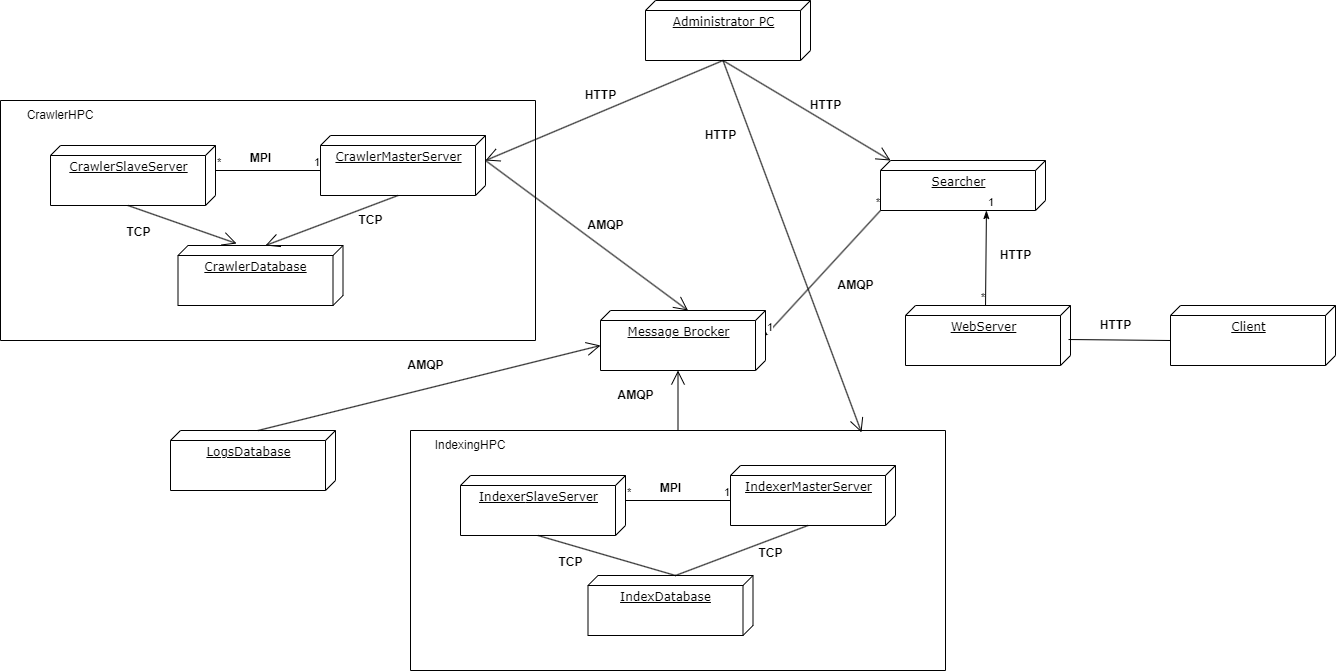
\includegraphics[width=1\linewidth]{diagram_deployment}}
\caption{Диаграмма развертывания распределенной поисковой системы}
\label{diagram_deployment:image}
\end{figure}

\subsection{Брокер сообщений}

Брокер сообщений -- программный компонент, который работает в качестве посредника между различными компонентами распределенной системы. 

Практически в любой реализации брокера сообщений выделяют следующие понятия: "<producer"> (отправитель) и "<consumer"> (потребитель или подписчик). Таким образом, брокер сообщений обрабатывает сообщения, полученные от отправителя, и перенаправляет их к соответствующим потребителям. Такой подход очень здорово уменьшает связность системы в целом, предоставляя хорошие перспективы для горизонтального масштабирования.

Как было сказано в разделе 3.3, брокером сообщений был выбран RabbitMQ на базе прикладного протокола передачи сообщений AMQP. Помимо понятий отправителя и потребителя, протоколом AMQP вводятся следующие важные в понимании работы RabbitMQ понятия:
\begin{itemize}
\item "<exchange"> (обменник) -- абстрактная промежуточная точка назначения отправленного сообщения;
\item "<queue"> (очередь) -- абстрактное хранилище сообщений;
\item "<routing key"> (ключ маршрутизации, маршрут) -- связующее звено ("<binding">) между обменником и очередью. Таким образом, пара из "<exchange"> и "<routing key"> однозначно определяет очередь назначения для отправленного сообщения.
\end{itemize}

На рисунке 3.2 представлена упрощенная схема работы RabbitMQ.
\begin{figure}[H]
\center{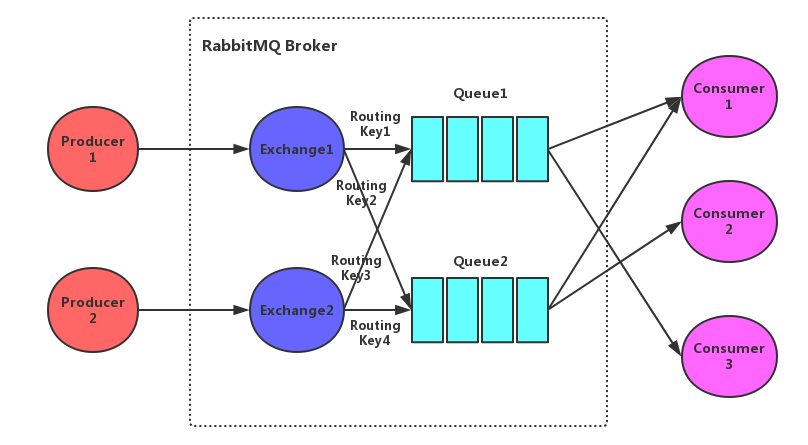
\includegraphics[width=1\linewidth]{rabbit_mq.png}}
\caption{Упрощенная схема работы RabbitMQ}
\label{rabbit_mq.png:image}
\end{figure}

В рамках проектирования распределенной системы необходимо определить доступные очереди, обменники и маршруты между ними.

В таблице 3.1 приведено описание очередей RabbitMQ.
\begin{xltabular}{\textwidth}{|X|X|X|X|}
	\caption{Описание очередей RabbitMQ}\label{mq_queues:table}\\ \hline
	\thead{Название} & \thead{Продолжительность} \\ \hline
	\thead{1} & \thead{2} \\ \hline
	\endfirsthead
	\continuecaption{Продолжение таблицы \ref{mq_queues:table}} \hline
	\thead{1} & \thead{2} \\ \hline
	\endhead
	pages\_to\_index & Durable \\ \hline
	resources\_ranks & Durable \\ \hline 
	logs & Durable \\ \hline
	queries & Durable \\ \hline
\end{xltabular}

В таблице 3.2 приведено описание обменников RabbitMQ.
\begin{xltabular}{\textwidth}{|X|X|X|X|}
	\caption{Описание обменников RabbitMQ}\label{mq_exchanges:table}\\ \hline
	\thead{Название} & \thead{Тип} & \thead{Продолжительность} \\ \hline
	\thead{1} & \thead{2} & \thead{3} \\ \hline
	\endfirsthead
	\continuecaption{Продолжение таблицы \ref{mq_exchanges:table}} \hline
	\thead{1} & \thead{2} & \thead{3} \\ \hline
	\endhead
	se & Direct & Durable \\ \hline
\end{xltabular}

В таблице 3.3 приведено описание маршрутов RabbitMQ.
\begin{xltabular}{\textwidth}{|X|X|X|X|}
	\caption{Описание маршрутов RabbitMQ}\label{mq_routes:table}\\ \hline
	\thead{Название\\обменника} & \thead{Название\\маршрута} & \thead{Название\\очереди} \\ \hline
	\thead{1} & \thead{2} & \thead{3} \\ \hline
	\endfirsthead
	\continuecaption{Продолжение таблицы \ref{mq_routes:table}} \hline
	\thead{1} & \thead{2} & \thead{3} \\ \hline
	\endhead
	se & pages\_to\_index & pages\_to\_index \\ \hline
	se & resources\_ranks & resources\_ranks \\ \hline
	se & logs & logs \\ \hline
	se & queries & queries \\ \hline
\end{xltabular}

\subsection{Поисковый робот}

Поисковый робот предназначен для обхода в ширину веб-графа, которым представлен Интернет. Он сохраняет метаинформацию о документах в базе данных до следующего обхода и переходит по их ссылкам с целью нахождения новых документов на заданном пространстве. После успешной валидация документ отправляется на шину данных для дальнейшей обработки другими компонентами, в частности, индексатором. 

\subsubsection{Типы обрабатываемых документов}
Робот при работе с ресурсами Интернета будет иметь дело со следующими типами документов:
\begin{itemize}
\item файл robots.txt, содержимое которое соответствует протоколу REP, не индексируется;
\item файлы навигации по веб-ресурсу в формате XML, содержимое которых соответствует протоколу SITEMAP, могут быть вложенными, не индексируются;
\item рядовые HTML-документы, которые должны быть проиндексированы системой и порождаются либо корневой страницей веб-ресурса, либо файлами навигации SITEMAP.
\end{itemize}

\subsubsection{Компоненты поискового робота}

На рисунке 3.3 представлена диаграмма компонентов поискового робота.

\begin{figure}[H]
\center{\includegraphics[width=1\linewidth]{robot/diagram_components}}
\caption{Диаграмма компонентов поискового робота распределенной системы}
\label{robot/diagram_components:image}
\end{figure}

\subsubsection{Описание базы данных}

В состав сущностей базы данных входят:
\begin{itemize}
\item «Methods» -- методы (протоколы) получения данных с ресурса;
\item «Domains» -- доменные имена ресурсов;
\item «ResourcesHeaders» -- заголовки ресурсов, включающие в себя метод получения данных и доменное имя;
\item «Resources» -- ресурсы, которые обходит робот.
\end{itemize}

В состав вышеперечисленных сущностей можно включить атрибуты, представленные в таблицах 3.4 – 3.7 соответственно.

\begin{xltabular}{\textwidth}{|X|X|X|X|}
	\caption{Спецификация сущности «Methods»}\label{crawler_methods:table}\\ \hline
	\thead{Поле} & \thead{Тип} & \thead{Обязат.} & \thead{Описание} \\ \hline
	\thead{1} & \thead{2} & \thead{3} & \thead{4} \\ \hline
	\endfirsthead
	\continuecaption{Продолжение таблицы \ref{crawler_methods:table}} \hline
	\thead{1} & \thead{2} & \thead{3} & \thead{4} \\ \hline
	\endhead
	Id & guid & + & Уникальный идентификатор метода \\ \hline
	Name & varchar & + & Название метода \\ \hline
\end{xltabular}

\begin{xltabular}{\textwidth}{|X|X|X|X|}
	\caption{Спецификация сущности «Domains»}\label{crawler_domains:table}\\ \hline
	\thead{Поле} & \thead{Тип} & \thead{Обязат.} & \thead{Описание} \\ \hline
	\thead{1} & \thead{2} & \thead{3} & \thead{4} \\ \hline
	\endfirsthead
	\continuecaption{Продолжение таблицы \ref{crawler_domains:table}} \hline
	\thead{1} & \thead{2} & \thead{3} & \thead{4} \\ \hline
	\endhead
	Id & guid & + & Уникальный идентификатор домена \\ \hline
	Name & varchar & + & Название домена \\ \hline
\end{xltabular}

\begin{xltabular}{\textwidth}{|X|X|X|X|}
	\caption{Спецификация сущности «ResourcesHeaders»}\label{crawler_resources_headers:table}\\ \hline
	\thead{Поле} & \thead{Тип} & \thead{Обязат.} & \thead{Описание} \\ \hline
	\thead{1} & \thead{2} & \thead{3} & \thead{4} \\ \hline
	\endfirsthead
	\continuecaption{Продолжение таблицы \ref{crawler_resources_headers:table}} \hline
	\thead{1} & \thead{2} & \thead{3} & \thead{4} \\ \hline
	\endhead
	Id & guid & + & Уникальный идентификатор заголовка \\ \hline
	MethodId & guid & + & Уникальный идентификатор метода \\ \hline
	DomainId & guid & + & Уникальный идентификатор домена \\ \hline
\end{xltabular}

\begin{xltabular}{\textwidth}{|X|X|X|X|}
	\caption{Спецификация сущности «Resources»}\label{crawler_resources:table}\\ \hline
	\thead{Поле} & \thead{Тип} & \thead{Обязат.} & \thead{Описание} \\ \hline
	\thead{1} & \thead{2} & \thead{3} & \thead{4} \\ \hline
	\endfirsthead
	\continuecaption{Продолжение таблицы \ref{crawler_resources:table}} \hline
	\thead{1} & \thead{2} & \thead{3} & \thead{4} \\ \hline
	\endhead
	Id & guid & + & Уникальный идентификатор ресурса \\ \hline
	Name & varchar & + & Название ресурса \\ \hline
	Checksum & varchar & + & SHA256-хеш содержимого ресурса \\ \hline
	Priority & double & + & Приоритет ресурса в обработке \\ \hline
	Fin & boolean & - & Флаг окончания обработки \\ \hline
\end{xltabular}

На рисунке 3.4 представлена ER-диаграмма базы данных поискового робота.

\begin{figure}[H]
\center{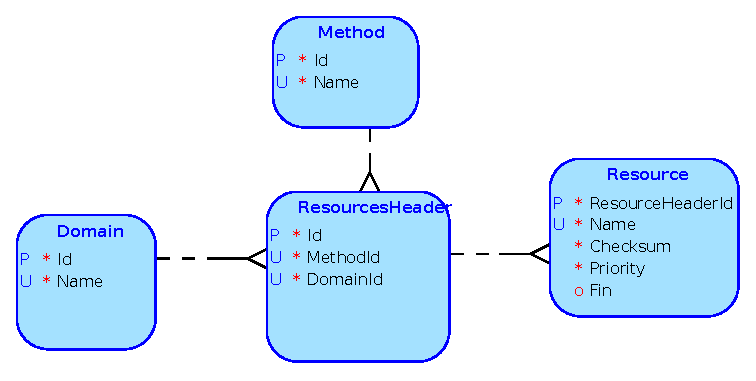
\includegraphics[width=1\linewidth]{robot/robot_db}}
\caption{ER-диаграмма базы данных поискового робота распределенной системы}
\label{robot/robot_db:image}
\end{figure}

\subsubsection{Описание потоков данных}

На рисунке 3.5 представлена диаграмма потоков данных для поискового робота распределенной системы.

\begin{figure}[H]
\center{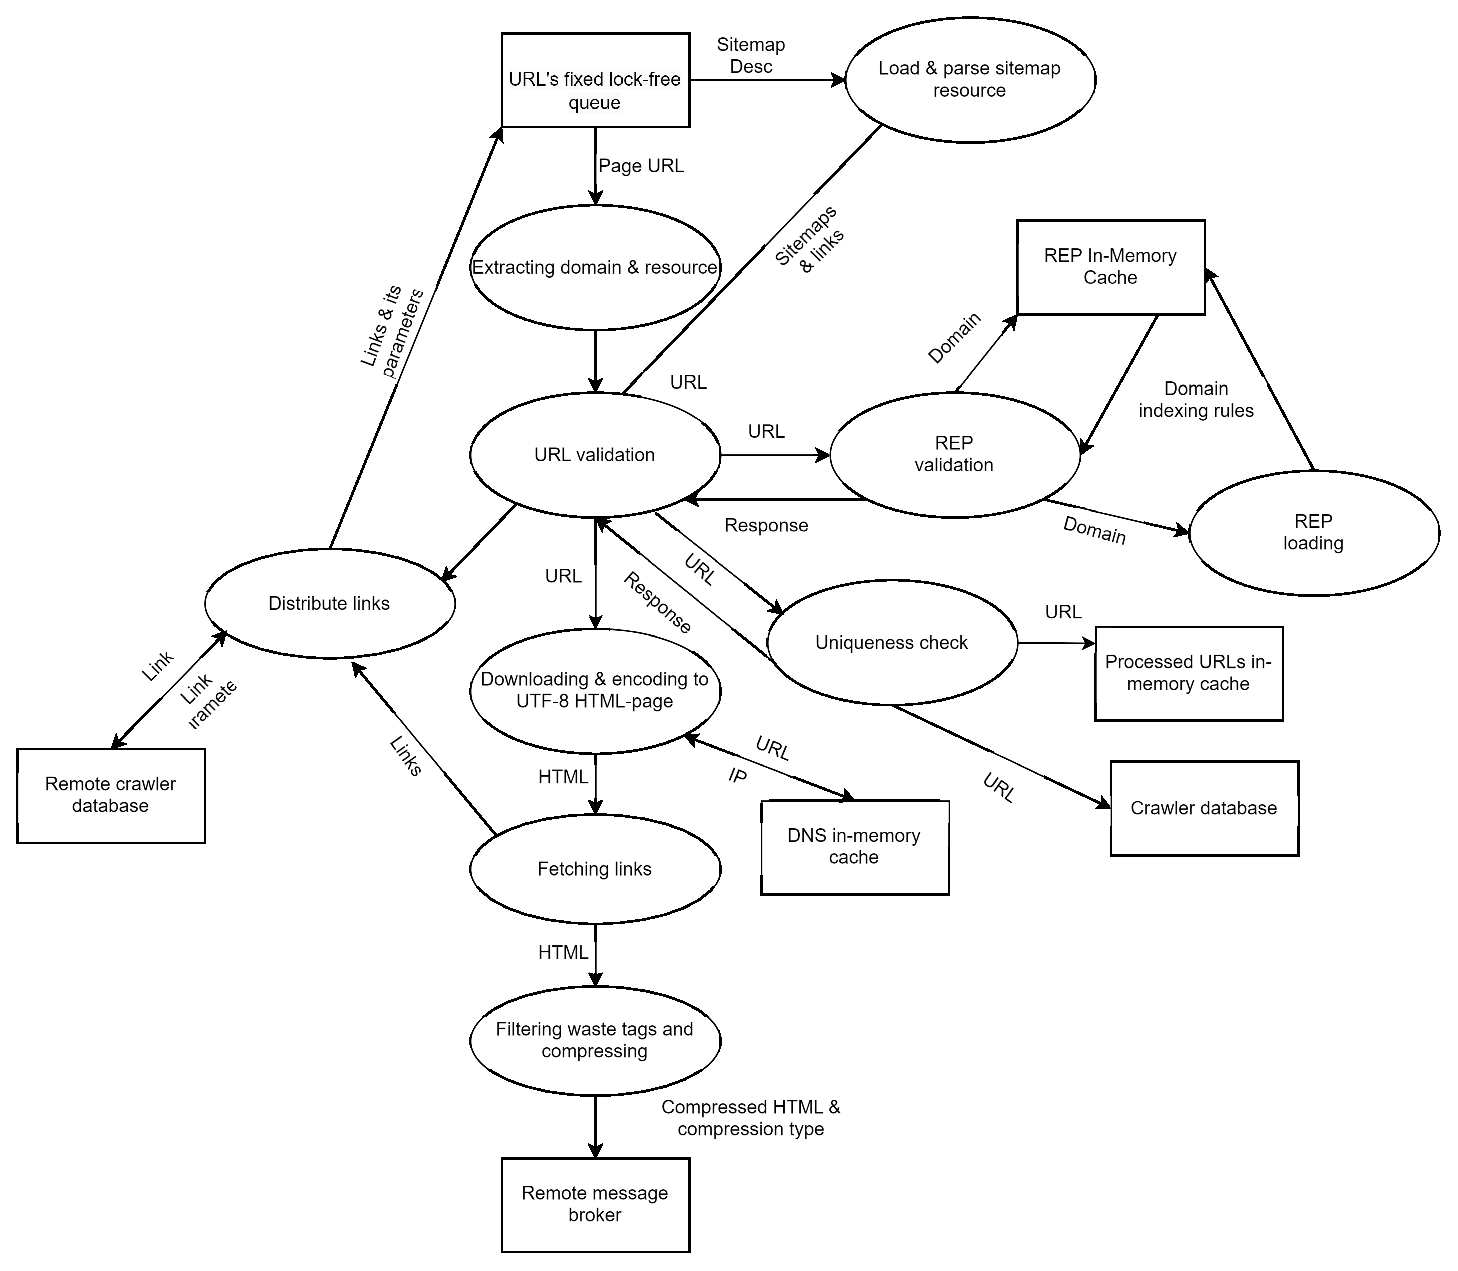
\includegraphics[width=1\linewidth]{robot/diagram_dataflow}}
\caption{Диаграмма потоков данных для поискового робота распределенной системы}
\label{robot/diagram_dataflow:image}
\end{figure}

\subsubsection{Описание концептуальных классов}

На рисунке 3.6 представлена диаграмма концептуальных классов для поискового робота распределенной системы.

\begin{figure}[H]
\center{\includegraphics[width=1\linewidth]{robot/diagram_classes}}
\caption{Диаграмма концептуальных классов для поискового робота распределенной системы}
\label{robot/diagram_classes:image}
\end{figure}

\subsubsection{Взаимодействие с брокером сообщений}

Компонент читает сообщения из следующих очередей:
\begin{itemize}
\item resources\_ranks.
\end{itemize}

В свою очередь, в таблице 3.8 представлено описание отправляемых сообщений.
\begin{xltabular}{\textwidth}{|X|X|X|X|}
	\caption{Описание отправляемых сообщений поискового робота}\label{crawler_bus_produce:table}\\ \hline
	\thead{Название\\обменника} & \thead{Название\\маршрута} & \thead{Сообщение\\JSON} \\ \hline
	\thead{1} & \thead{2} & \thead{3} \\ \hline
	\endfirsthead
	\continuecaption{Продолжение таблицы \ref{crawler_bus_produce:table}} \hline
	\thead{1} & \thead{2} & \thead{3} \\ \hline
	\endhead
	se & pages\_to\_index & \{"url": "string"\, "content": "string"\} \\ \hline
\end{xltabular}

\subsection{Индексатор}

Индексатор - компонент системы, ответственный за статический анализ полученных им документов, результаты которого впоследствии будут использоваться в режиме чтения поисковиком. 
При проектировании и разработке индексатора сосредоточимся на следующих главных задачах:
\begin{itemize}
\item обеспечение контроля сбора ресурсов из брокера сообщений;
\item разработка алгоритма индексирования документов;
\item разработка алгоритма вычисления статического ранга документов.
\end{itemize}

\subsubsection{Описание контроля сбора ресурсов}
Контроль сбора ресурсов будет включать в себя следующие обязательные аспекты:
\begin{itemize}
\item ограничение количества ресурсов для индексирования. После предварительной обработки некоторого натурального числа документов сбор новых прекращается и начинаются следующие стадии индексации;
\item парциальный сбор ресурсов. Ввиду того, что предварительная индексация ресурса выполняется намного дольше, чем его получение из очереди сообщений, разумно делать это парциально, чтобы в конечном итоге не перегрузить оперативную память. По этой причине индексатору будет задаваться размер порции ресурсов для обработки и желаемая скорость в единицах в секунду.
\end{itemize}

\subsubsection{Индексирование документов}

Логической моделью проиндексированных документов будет являться инвертированный индекс. 

Инвертированный индекс - индекс, который представляет собой хеш-таблицу следующей конфигурации: 
\begin{itemize}
\item ключом является термин, как правило, его глобальный целочисленный индентификатор;
\item значение же представляется в виде списка глобальных идентификаторов документов, в которых данный термин был встречен хотя бы один раз.
\end{itemize}

Однако одной лишь структуры мало. Терминов в одном документе может быть много, поэтому необходимо для каждого из них рассчитать их относительный ранг, находящийся в диапазоне от 0 до 1 включительно. Этот ранг будет вычисляться на основе абсолютной взвешенной частоты термина и его обратной документной частоты.

Кроме того, в целях повышения производительности системы организуем индекс так, чтобы поиск по нему мог осуществляться нечетко, но с минимальными потерями в точности и полноте поиска. Этого можно достичь с использованием так называемых "<чемпионских списков">.

Чемпионские списки представляют из себя хеш-таблицу, где ключом выступает целочисленный идентификатор термина, а значением - ограниченный в размере список идентификаторов документов, расположенных по убыванию, начиная с документа, в котором заданный термин имеет максимальный относительный ранг. 

\paragraph{Абсолютная взвешенная частота термина}

Абсолютная взвешенная частота функционально зависит от количество вхождений термина в документ. Но так как мы зачастую будем иметь дело с форматами данных древовидной структуры, таких как HTML, мы можем дополнительно присваивать каждому типу узла свой вес $w$. Кроме того, чтобы учитывать вложенность узлов, необходимо ввести агрегирующую весовую функцию $Agg$. Итак, полная формула вычисления абсолютной взвешенной частоты термина в документе принимает следующий вид:

\begin{equation}
WTF(t) = \sum_{i = 1}^{n}Agg(w_1, w_2, ..., w_m)
\end{equation} где $n$ -- количество вхождений термина данных, а $m$ -- количество взвешенных предков-узлов элемента, в содержание текста которого входит термин $t$.

Смысл абсолютной взвешенной частоты термина достаточно прост. Чем чаще термин встречается в документе, тем выше его последующий ранг. Однако нередки случаи, когда высокая внутридокументная частота термина обусловлена лишь тем, что этот термин входит в число частоиспользуемых. Чтобы снизить влияние данного фактора, вводится понятие обратной документной частоты термина.

\paragraph{Обратная документная частота термина}

Документная частота термина ($DTF$) - количество документов, в которых термин был встречен хотя бы один раз. Обратная документная частота же определяется следующим образом:

\begin{equation}
IDTF(t) = \log\frac{N}{DTF(t)}
\end{equation} где $N$ -- общее количество документов, $DTF(t)$ -- документная частота термина $t$.

Смысл обратной документной частоты заключается в том, что в случае, если термин встречается в большом количестве документов, то независимо от $WTF$ ранг термина будет снижен.

\paragraph{Относительный ранг термина в документе}

Абсолютный ранг термина в документе вычисляется следующим образом:
\begin{equation}
ATR(t) = WTF(t) * IDTF(t)
\end{equation}

В свою очередь, относительный ранг термина вычисляется путем нормализации её абсолютных вариаций:
\begin{equation}
RTR(t) = \frac{ATR(t)}{\sqrt(\sum{i = 1}^{n}ATR(t_1)^2 + ATR(t_2)^2 + ... + ATR(t_m)^2)}
\end{equation} где $m$ -- количество различных терминов в документе.

\subsubsection{Статическое ранжирование документов}

С целью повышения релевантности поисковой выдачи необходимо учитывать конфигурацию веб-графа документов в целом. Поэтому разумно каждому документы присвоить некоторый относительный ранг, который будет зависеть от количества и качества входящих и исходящих ссылок. Интуитивно очевидно, что ранг документа должен быть выше, если выше вероятность перехода на него по гиперссылке. В таком случае мы можем представить документы, как состояния марковской цепи. 

Марковская цепь -- это дискретный стохастический процесс, представляющий собой последовательность временных шагов, на каждом из которых происходит случайн выбор независимо от предыдущего.

Марковская цепь характеризуется матрицей вероятностей переходов $P$, имеющей размерность $N$ x $N$, где $N$ - количество состояний цепи. Сумма элементов в строке матрицы переходов должна равняться 1. В таком случае $P(i, j)$ - вероятность перехода с $i$-ой страницы на $j$-ую.

Матрица с неотрицательными элементами называется стохастической. Ключевое её свойство заключается в том, что она имеет главный левый собственный вектор, соответствующий максимальному значению, которое равно единице.

Также введем определение эргодической марковской цепи.

Марковская цепь называется эргодической, если существует положительное целове число $T_0$, такое. что для всех пар состояний $i$, $j$ в марковской цепи, стартующей в момент $t = 0$ из состояния $i$, для всех $t > T_0$ вероятность нахождения в момент времени $t$ в состоянии $j$ больше нуля.

Иными словами для эргодической марковской цепи должны быть выполнены следующие условия:
\begin{itemize}
\item неразложимость -- гарантирует, что существует последовательность переходов с ненулевой вероятностью из любого состояния в любое другое;
\item апериодичность -- гарантирует, что состояния не делятся на такие множества, что все переходы осуществляются циклически из состояний одного множества в состояния другого множества.
\end{itemize}

И, наконец, для любой эргодической цепи верно следующее утверждение.

Для любой эргодической цепи Маркова существует единственный вектор стационарного распределения вероятностей $\vec{p}$, являющийся главным левым собственным вектором матрицы $P$, и если $f(i, t)$ -- количество переходов в состоянии $i$ за $t$ шагов, то 

\begin{equation}
lim_{t \to \inf}\frac{f(i, t)}{t}=p(i)
\end{equation} где $p(i) > 0$ -- стационарная вероятность состояния $i$.

Чтобы воспользоваться вышеописанное теоретической выкладкой, сформируем модель обхода документов.

Пусть есть некоторый абстрактный "<путешественник">, который в случайном порядке переходит со страницы на страницу.
Определим два несовместных типа переходов:
\begin{itemize}
\item стационарный переход с одной страницы на другую по гиперссылке, который имеет свою вероятностную оценку;
\item телепортация с постоянной вероятностью $\alpha$ c одной страницы на другую не задействуя гиперссылки. Такая возможность сделает нашу марковскую цепь эргодической.
\end{itemize}

Итак, формула полной вероятности перехода с $i$-ой страницы на $j$-ую будет иметь вид:

\begin{equation}
P(i, j) = \frac{1}{L_i} * (1 - \alpha) + \frac{1}{N} * \alpha
\end{equation} где $L_i$ -- количество ненулевых элементов матрицы смежности веб-графа на строке $i$, $N$ -- общее количество документов.

На основе этой формулы мы формируем матрицу вероятностных переходов марковской эргодической цепи и итеративно приближенно вычисляем её левый собственный вектор, который будет являться стационарным распределением вероятностей между всеми документами из множества, что мы и будем называть статическим рангом документа.

\subsubsection{Описание алгоритма индексирования}

Алгоритм индексирования будет иметь три логические стадии:
\begin{enumerate}
\item Стадия первичного индексирования, в ходе которой происходит загрузка информации о ресурсах из шины данных и их первичная обработка, которая состоит из следующих шагов:
\begin{enumerate}
\item Проверка документа на уникальность. В случае, если подобный документ уже был обработан, процесс переходит к следующему документу из очереди.
\item Сжатие содержимого документа по заданному алгоритму, его запись в базу данных и получение целочисленного идентификатора документа.
\item Парсинг документа на массив взвешенных терминов. В данном случае вес токена -- абсолютная взвешенная частота термина в документе.
\item Запись новых терминов в базу данных и получение целочисленных идентификаторов терминов.
\item Запись в таблицу-связь с документами и терминами кортежей вида ("<идентификатор документа">, "<идентификатор термина">, "<абсолютная взвешенная частота термина">).
\end{enumerate}
\item Стадия вторичного индексирования. Она начинается после окончания чтения новых ресурсов из шины данных при достижении определенного количества и обработки всех документов из очереди. В течение этой стадии будут происходить следующие подэтапы, некоторые из которых могут выполняться параллельно друг другу:
\begin{enumerate}
\item Для каждой пары ("<документ">, "<термин">) будет вычисляться относительный ранг вхождения этого термина в документа на основе вышеприведенных формул.
\item Создание чемпионских списков (зависит от п.1).
\item Вычисление элементов вероятностной матрицы переходов в рамках полученного подграфа всего веб-графа.
\item Вычисление статического ранга документов на основе вероятностной матрицы переходов (зависит от п.3).
\item Отправка статических рангов обработанных страниц на шину данных (зависит от п.4).
\end{enumerate}
\item Синхронизация. В ходе этой стадии данные старого индекса будут перезаписаны новосозданным.
\end{enumerate}

\subsubsection{Компоненты индексатора}

На рисунке 3.7 представлена диаграмма компонентов индексатора.

\begin{figure}[H]
\center{\includegraphics[width=1\linewidth]{indexer/diagram_components}}
\caption{Диаграмма компонентов индексатора распределенной поисковой системы}
\label{indexer/diagram_components:image}
\end{figure}

\subsubsection{Описание базы данных}

Модель данных будет состоять из двух логических частей, физически расположенных в одной базе:
\begin{enumerate}
\item Эталонная часть модели, предназначенная исключительно для чтения поисковиком при обработке пользовательских запросов;
\item Черновая часть модели, предназначенная для создания новых версий индекса, не вмешиваясь во внутреннюю структуру эталонной модели. Она содержит в себе полную копию структуры эталонной модели с несколькими дополнениями, необходимыми для эффективного создания индекса. После завершения создания черновой модели она атомарно целиком заменяет эталонную, при этом полностью очищаясь для создания следующего экземпляра индекса.
\end{enumerate}

В состав сущностей базы данных входят:
\begin{itemize}
\item «Methods» -- методы (протоколы) получения данных с ресурса (эталон);
\item «MethodsSec» -- методы (протоколы) получения данных с ресурса (черновик);
\item «Domains» -- доменные имена ресурсов (эталон);
\item «DomainsSec» -- доменные имена ресурсов (черновик);
\item «ResourcesHeaders» -- заголовки ресурсов, включающие в себя метод получения данных и доменное имя (эталон);
\item «ResourcesHeadersSec» -- заголовки ресурсов, включающие в себя метод получения данных и доменное имя (черновик);
\item «Resources» -- ресурсы, которые входят в индекс системы (эталон);
\item «ResourcesSec» -- ресурсы, которые входят в индекс системы (черновик);
\item «Lexems» -- информация о лексемах, полученных с ресурсов (эталон);
\item «LexemsSec» -- нформация о лексемах, полученных с ресурсов (черновик);
\item «ResourcesLexems» -- информация о лексемах в содержимом ресурсов (эталон);
\item «ResourcesLexemsSec» -- нформация о лексемах в содержимом ресурсов (черновик);
\item «ChampionLists» -- чемпионские списки для каждой лексемы (эталон);
\item «ChampionListsSec» -- емпионские списки для каждой лексемы (черновик);
\item «ResourcesAdhacencySec» -- представление вероятностной матрицы смежности ресурсов;
\item «TemporaryResourceRanksSec» -- промежуточное хранилище рангов ресурсов.
\end{itemize}

В состав вышеперечисленных сущностей можно включить атрибуты, представленные в таблицах 3.9 – 3.24 соответственно.

\begin{xltabular}{\textwidth}{|X|X|X|X|}
	\caption{Спецификация сущности «Methods»}\label{indexer_methods:table}\\ \hline
	\thead{Поле} & \thead{Тип} & \thead{Обязат.} & \thead{Описание} \\ \hline
	\thead{1} & \thead{2} & \thead{3} & \thead{4} \\ \hline
	\endfirsthead
	\continuecaption{Продолжение таблицы \ref{indexer_methods:table}} \hline
	\thead{1} & \thead{2} & \thead{3} & \thead{4} \\ \hline
	\endhead
	Id & integer & + & Уникальный идентификатор метода \\ \hline
	Name & varchar & + & Название метода \\ \hline
\end{xltabular}

\begin{xltabular}{\textwidth}{|X|X|X|X|}
	\caption{Спецификация сущности «MethodsSec»}\label{indexer_methods_sec:table}\\ \hline
	\thead{Поле} & \thead{Тип} & \thead{Обязат.} & \thead{Описание} \\ \hline
	\thead{1} & \thead{2} & \thead{3} & \thead{4} \\ \hline
	\endfirsthead
	\continuecaption{Продолжение таблицы \ref{indexer_methods_sec:table}} \hline
	\thead{1} & \thead{2} & \thead{3} & \thead{4} \\ \hline
	\endhead
	Id & integer & + & Уникальный идентификатор метода \\ \hline
	Name & varchar & + & Название метода \\ \hline
\end{xltabular}

\begin{xltabular}{\textwidth}{|X|X|X|X|}
	\caption{Спецификация сущности «Domains»}\label{indexer_domains:table}\\ \hline
	\thead{Поле} & \thead{Тип} & \thead{Обязат.} & \thead{Описание} \\ \hline
	\thead{1} & \thead{2} & \thead{3} & \thead{4} \\ \hline
	\endfirsthead
	\continuecaption{Продолжение таблицы \ref{indexer_domains:table}} \hline
	\thead{1} & \thead{2} & \thead{3} & \thead{4} \\ \hline
	\endhead
	Id & integer & + & Уникальный идентификатор домена \\ \hline
	Name & varchar & + & Название домена \\ \hline
\end{xltabular}

\begin{xltabular}{\textwidth}{|X|X|X|X|}
	\caption{Спецификация сущности «DomainsSec»}\label{indexer_domains_sec:table}\\ \hline
	\thead{Поле} & \thead{Тип} & \thead{Обязат.} & \thead{Описание} \\ \hline
	\thead{1} & \thead{2} & \thead{3} & \thead{4} \\ \hline
	\endfirsthead
	\continuecaption{Продолжение таблицы \ref{indexer_domains_sec:table}} \hline
	\thead{1} & \thead{2} & \thead{3} & \thead{4} \\ \hline
	\endhead
	Id & integer & + & Уникальный идентификатор домена \\ \hline
	Name & varchar & + & Название домена \\ \hline
\end{xltabular}

\begin{xltabular}{\textwidth}{|X|X|X|X|}
	\caption{Спецификация сущности «ResourcesHeaders»}\label{indexer_resources_headers:table}\\ \hline
	\thead{Поле} & \thead{Тип} & \thead{Обязат.} & \thead{Описание} \\ \hline
	\thead{1} & \thead{2} & \thead{3} & \thead{4} \\ \hline
	\endfirsthead
	\continuecaption{Продолжение таблицы \ref{indexer_resources_headers:table}} \hline
	\thead{1} & \thead{2} & \thead{3} & \thead{4} \\ \hline
	\endhead
	Id & integer & + & Уникальный идентификатор заголовка \\ \hline
	MethodId & integer & + & Уникальный идентификатор метода \\ \hline
	DomainId & integer & + & Уникальный идентификатор домена \\ \hline
\end{xltabular}

\begin{xltabular}{\textwidth}{|X|X|X|X|}
	\caption{Спецификация сущности «ResourcesHeadersSec»}\label{indexer_resources_headers_sec:table}\\ \hline
	\thead{Поле} & \thead{Тип} & \thead{Обязат.} & \thead{Описание} \\ \hline
	\thead{1} & \thead{2} & \thead{3} & \thead{4} \\ \hline
	\endfirsthead
	\continuecaption{Продолжение таблицы \ref{indexer_resources_headers_sec:table}} \hline
	\thead{1} & \thead{2} & \thead{3} & \thead{4} \\ \hline
	\endhead
	Id & integer & + & Уникальный идентификатор заголовка \\ \hline
	MethodId & integer & + & Уникальный идентификатор метода \\ \hline
	DomainId & integer & + & Уникальный идентификатор домена \\ \hline
\end{xltabular}

\begin{xltabular}{\textwidth}{|X|X|X|X|}
	\caption{Спецификация сущности «Resources»}\label{indexer_resources:table}\\ \hline
	\thead{Поле} & \thead{Тип} & \thead{Обязат.} & \thead{Описание} \\ \hline
	\thead{1} & \thead{2} & \thead{3} & \thead{4} \\ \hline
	\endfirsthead
	\continuecaption{Продолжение таблицы \ref{indexer_resources:table}} \hline
	\thead{1} & \thead{2} & \thead{3} & \thead{4} \\ \hline
	\endhead
	Id & bigint & + & Уникальный идентификатор ресурса \\ \hline
	ResourceHeaderId & integer & + & Уникальный идентификатор заголовка ресурса \\ \hline 
	Name & varchar & + & Название ресурса \\ \hline
	Title & varchar & + & Заголовок ресурса \\ \hline
	CompressionType & varchar & - & Тип сжатия содержимого в базе данных \\ \hline
	Content & binary & + & Сжатое содержимое ресурса \\ \hline
	Size & integer & + & Размер исходного содержимого ресурса в байтах \\ \hline
\end{xltabular}

\begin{xltabular}{\textwidth}{|X|X|X|X|}
	\caption{Спецификация сущности «ResourcesSec»}\label{indexer_resources_sec:table}\\ \hline
	\thead{Поле} & \thead{Тип} & \thead{Обязат.} & \thead{Описание} \\ \hline
	\thead{1} & \thead{2} & \thead{3} & \thead{4} \\ \hline
	\endfirsthead
	\continuecaption{Продолжение таблицы \ref{indexer_resources_sec:table}} \hline
	\thead{1} & \thead{2} & \thead{3} & \thead{4} \\ \hline
	\endhead
	Id & bigint & + & Уникальный идентификатор ресурса \\ \hline
	ResourceHeaderId & integer & + & Уникальный идентификатор заголовка ресурса \\ \hline 
	Name & varchar & + & Название ресурса \\ \hline
	Title & varchar & + & Заголовок ресурса \\ \hline
	CompressionType & varchar & - & Тип сжатия содержимого в базе данных \\ \hline
	Content & binary & + & Сжатое содержимое ресурса \\ \hline
	Size & integer & + & Размер исходного содержимого ресурса в байтах \\ \hline
\end{xltabular}

\begin{xltabular}{\textwidth}{|X|X|X|X|}
	\caption{Спецификация сущности «Lexems»}\label{indexer_lexems:table}\\ \hline
	\thead{Поле} & \thead{Тип} & \thead{Обязат.} & \thead{Описание} \\ \hline
	\thead{1} & \thead{2} & \thead{3} & \thead{4} \\ \hline
	\endfirsthead
	\continuecaption{Продолжение таблицы \ref{indexer_lexems:table}} \hline
	\thead{1} & \thead{2} & \thead{3} & \thead{4} \\ \hline
	\endhead
	Id & integer & + & Уникальный идентификатор лексемы \\ \hline
	Name & varchar & + & Название лексемы \\ \hline
	Language & varchar & + & Язык лексемы \\ \hline
	Df & bigint & + & Документная частота лексемы \\ \hline
\end{xltabular}

\begin{xltabular}{\textwidth}{|X|X|X|X|}
	\caption{Спецификация сущности «LexemsSec»}\label{indexer_lexems_sec:table}\\ \hline
	\thead{Поле} & \thead{Тип} & \thead{Обязат.} & \thead{Описание} \\ \hline
	\thead{1} & \thead{2} & \thead{3} & \thead{4} \\ \hline
	\endfirsthead
	\continuecaption{Продолжение таблицы \ref{indexer_lexems_sec:table}} \hline
	\thead{1} & \thead{2} & \thead{3} & \thead{4} \\ \hline
	\endhead
	Id & integer & + & Уникальный идентификатор лексемы \\ \hline
	Name & varchar & + & Название лексемы \\ \hline
	Language & varchar & + & Язык лексемы \\ \hline
	Df & bigint & + & Документная частота лексемы \\ \hline
\end{xltabular}

\begin{xltabular}{\textwidth}{|X|X|X|X|}
	\caption{Спецификация сущности «ResourcesLexems»}\label{indexer_resources_lexems:table}\\ \hline
	\thead{Поле} & \thead{Тип} & \thead{Обязат.} & \thead{Описание} \\ \hline
	\thead{1} & \thead{2} & \thead{3} & \thead{4} \\ \hline
	\endfirsthead
	\continuecaption{Продолжение таблицы \ref{indexer_resources_lexems:table}} \hline
	\thead{1} & \thead{2} & \thead{3} & \thead{4} \\ \hline
	\endhead
	ResourceId & bigint & + & Уникальный идентификатор ресурса \\ \hline
	LexemId & integer & + & Уникальный идентификатор лексемы \\ \hline
	Wtf & double & + & Абсолютная взвешенная частота лексемы в содержимом ресурса \\ \hline
	Rank & double & + & Относительный ранг лексемы в содержимом текущего ресурса \\ \hline
\end{xltabular}

\begin{xltabular}{\textwidth}{|X|X|X|X|}
	\caption{Спецификация сущности «ResourcesLexemsSec»}\label{indexer_resources_lexems_sec:table}\\ \hline
	\thead{Поле} & \thead{Тип} & \thead{Обязат.} & \thead{Описание} \\ \hline
	\thead{1} & \thead{2} & \thead{3} & \thead{4} \\ \hline
	\endfirsthead
	\continuecaption{Продолжение таблицы \ref{indexer_resources_lexems_sec:table}} \hline
	\thead{1} & \thead{2} & \thead{3} & \thead{4} \\ \hline
	\endhead
	ResourceId & bigint & + & Уникальный идентификатор ресурса \\ \hline
	LexemId & integer & + & Уникальный идентификатор лексемы \\ \hline
	Wtf & double & + & Абсолютная взвешенная частота лексемы в содержимом ресурса \\ \hline
	Rank & double & + & Относительный ранг лексемы в содержимом текущего ресурса \\ \hline
\end{xltabular}

\begin{xltabular}{\textwidth}{|X|X|X|X|}
	\caption{Спецификация сущности «ChampionLists»}\label{indexer_champion_lists:table}\\ \hline
	\thead{Поле} & \thead{Тип} & \thead{Обязат.} & \thead{Описание} \\ \hline
	\thead{1} & \thead{2} & \thead{3} & \thead{4} \\ \hline
	\endfirsthead
	\continuecaption{Продолжение таблицы \ref{indexer_champion_lists:table}} \hline
	\thead{1} & \thead{2} & \thead{3} & \thead{4} \\ \hline
	\endhead
	LexemId & integer & + & Уникальный идентификатор лексемы \\ \hline
	ResourcesId & array[bigint] & + & Массив идентификаторов ресурсов \\ \hline
\end{xltabular}

\begin{xltabular}{\textwidth}{|X|X|X|X|}
	\caption{Спецификация сущности «ChampionListsSec»}\label{indexer_champion_lists_sec:table}\\ \hline
	\thead{Поле} & \thead{Тип} & \thead{Обязат.} & \thead{Описание} \\ \hline
	\thead{1} & \thead{2} & \thead{3} & \thead{4} \\ \hline
	\endfirsthead
	\continuecaption{Продолжение таблицы \ref{indexer_champion_lists_sec:table}} \hline
	\thead{1} & \thead{2} & \thead{3} & \thead{4} \\ \hline
	\endhead
	LexemId & integer & + & Уникальный идентификатор лексемы \\ \hline
	ResourcesId & array[bigint] & + & Массив идентификаторов ресурсов \\ \hline
\end{xltabular}

\begin{xltabular}{\textwidth}{|X|X|X|X|}
	\caption{Спецификация сущности «ResourcesAdjacencySec»}\label{indexer_resources_adjacency_sec:table}\\ \hline
	\thead{Поле} & \thead{Тип} & \thead{Обязат.} & \thead{Описание} \\ \hline
	\thead{1} & \thead{2} & \thead{3} & \thead{4} \\ \hline
	\endfirsthead
	\continuecaption{Продолжение таблицы \ref{indexer_resources_adjacency_sec:table}} \hline
	\thead{1} & \thead{2} & \thead{3} & \thead{4} \\ \hline
	\endhead
	IdFrom & bigint & + & Уникальный идентификатор ресурса-отправителя \\ \hline
	IdTo & integer & + & Уникальный идентификатор ресурса-назначения \\ \hline
	Probability & double & + & Вероятность перехода \\ \hline
\end{xltabular}

\begin{xltabular}{\textwidth}{|X|X|X|X|}
	\caption{Спецификация сущности «TemporaryResourceRanksSec»}\label{indexer_temp_resource_ranks_sec:table}\\ \hline
	\thead{Поле} & \thead{Тип} & \thead{Обязат.} & \thead{Описание} \\ \hline
	\thead{1} & \thead{2} & \thead{3} & \thead{4} \\ \hline
	\endfirsthead
	\continuecaption{Продолжение таблицы \ref{indexer_temp_resource_ranks_sec:table}} \hline
	\thead{1} & \thead{2} & \thead{3} & \thead{4} \\ \hline
	\endhead
	ResourceId & bigint & + & Уникальный идентификатор ресурса \\ \hline
	Rank & double & - & Ранг ресурса \\ \hline
\end{xltabular}

На рисунках 3.8 - 3.9 представлены ER-диаграммы эталонной и черновой части базы данных индекса распределенной системы.

\begin{figure}[H]
\center{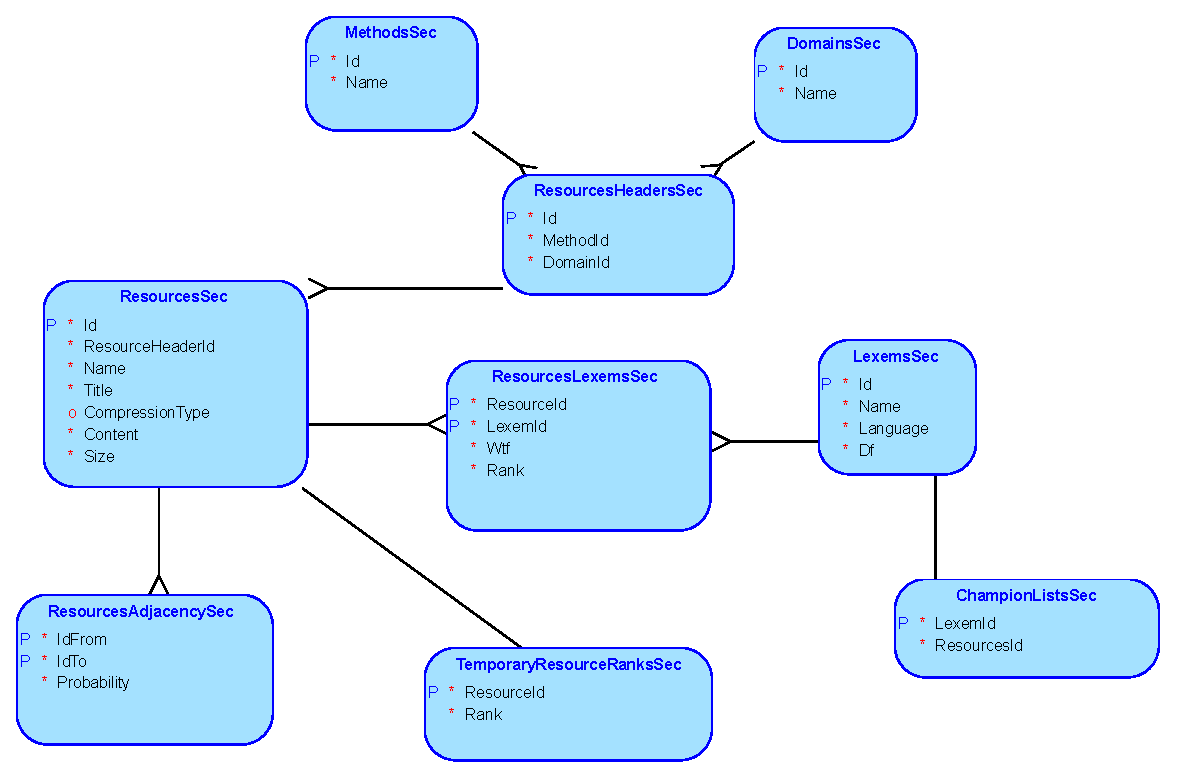
\includegraphics[width=1\linewidth]{indexer/indexer_sec_db}}
\caption{ER-диаграмма черновой части базы данных индексатора распределенной системы}
\label{indexer/indexer_sec_db:image}
\end{figure}
\begin{figure}[H]
\center{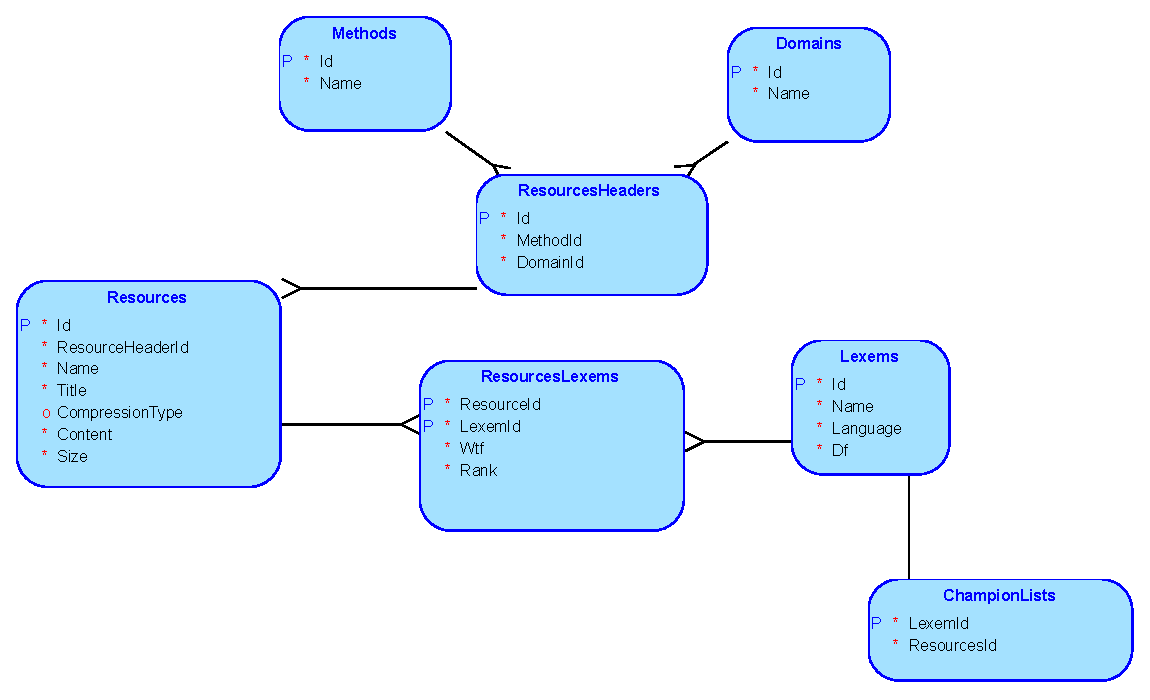
\includegraphics[width=1\linewidth]{indexer/indexer_db}}
\caption{ER-диаграмма эталонной части базы данных индексатора распределенной системы}
\label{indexer/indexer_db:image}
\end{figure}

\subsubsection{Описание концептуальных классов}

На рисунке 3.10 представлена диаграмма концептуальных классов для индексатора распределенной системы.
\begin{figure}[H]
\center{\includegraphics[width=1\linewidth]{indexer/diagram_classes}}
\caption{Диаграмма концептуальных классов для индексатора распределенной системы}
\label{indexer/diagram_classes:image}
\end{figure}

\subsubsection{Взаимодействие с брокером сообщений}

Компонент читает сообщения из следующих очередей:
\begin{itemize}
\item pages\_to\_index.
\end{itemize}

В свою очередь, в таблице 3.25 представлено описание отправляемых сообщений.
\begin{xltabular}{\textwidth}{|X|X|X|X|}
	\caption{Описание отправляемых сообщений индексатора}\label{indexer_bus_produce:table}\\ \hline
	\thead{Название\\обменника} & \thead{Название\\маршрута} & \thead{Сообщение\\JSON} \\ \hline
	\thead{1} & \thead{2} & \thead{3} \\ \hline
	\endfirsthead
	\continuecaption{Продолжение таблицы \ref{indexer_bus_produce:table}} \hline
	\thead{1} & \thead{2} & \thead{3} \\ \hline
	\endhead
	se & resources\_ranks & \{"url": "string"\, "rank": "double"\} \\ \hline
\end{xltabular}

\subsection{Поисковик}

Поисковик предназначен для обработки пользовательских запросов и выдачи релеватных результатов поиска с помощью ранее созданного индекса документов.

\subsubsection{Описание процесса ранжирования документов}

Начнем с того, что заметим, что количество всех веб-документов хоть и велико, но ограничено некоторым натуральным числом. По этой причине количество возможных терминов также ограничено некоторым натуральным числом $T$. 

Следовательно, множество всех веб-документов можно рассмотреть, как конечное векторное пространство размерности $T$. 

В свою очередь, каждый документ определяется некоторым вектором
\begin{equation}
\vec{D}=(r_1, r_2, ..., r_T)
\end{equation} где $r_i$ -- относительный ранг термина с номером $i$ в документе $D$.

Мерой соответствия одного документа другому можно считать косинус угла между их векторами в вышеопределенном векторном пространстве, а именно следующее:

\begin{equation}
R(d_1, d_2)=\frac{\vec{d_1} * \vec{d_2}}{|\vec{d_1}| |\vec{d_2}|}
\end{equation} где $R$ -- мера соответствия документа $d_1$ документу $d_2$ и наоборот.

Пользовательский запрос будет рассматриваться системой как документ, так как фактически тоже имеет своё текстовое значение и определенную смысловую нагрузку. Поэтому для получения меры соответствия запроса какому-либо документу, будет необходимо получить вектор запроса и найти значение косинуса угла между ним и вектором целевого документа.

\subsubsection{Описание алгоритма работы поисковика}
Алгоритм работы поисковика состоит в следующем:
\begin{enumerate}
\item Анализ и разбиение возможного мультиязычного пользовательского запроса на множество отрывков с одинаковым языком. В зависимости от вероятности соответствия предсказанного языка к отрывку присвоить каждому из них свой первоначальный ранг. Добиться подобного функционала можно с использованием нейросетей.
\item С помощью парсера свободных текстовых запросов разбить отрывки на множество лексем в соответствие с правилами. В рамках данной работы предполагаются следующие действия:
\begin{itemize}
\item фильтрация стоп-слов (часто употребимых слов для каждого языка, которые не несут существенной смысловой нагрузки);
\item операция стемминга для присвоения каждой лексемы к конкретному классу эквивалентности.
\end{itemize}
\item Объединить множества лексем из всех отрывков в один большой поток токенов. Пользовательский запрос будет рассматриваться как документ, поэтому каждый токен будет иметь свою взвешенную частотную характеристику, название языка и непосредственно значение. Так как документ всего один - запрос, то в этом случае взвешенная частотная характеристика совпадает с абсолютным рангом токена. По этой причине остается провести лишь операцию нормализации рангов, с целью для каждого термина получить относительный ранг.
\item Получив векторное представление пользовательского запроса, для каждого его термина найдем чемпионские списки и объединим их, получив в конечном итоге целевое множество документов для поиска.
\item Для каждого документа находится косинусная мера его соответствия пользовательскому запросу. По итогу для каждого документа мы имеем $\vec{R}$, у которого есть две составляющие: косинусная мера соответствия запросу (динамическая) и ранг (статическая).
\item С помощью заданного коэффициента приоритета статического критерия над динамическим объединяем две составляющие через нахождение длины $\vec{R}$, будем считать это релевантностью документа.
\item Сортируем документы по убыванию релевантности и отправляем заголовок, URL и релевантность документа в соответствие с заданными параметрами смещения и количества.
\end{enumerate}

\subsubsection{Компоненты поисковика}

На рисунке 3.11 представлена диаграмма компонентов поисковика распределенной системы.

\begin{figure}[H]
\center{\includegraphics[width=1\linewidth]{searcher/diagram_components}}
\caption{Диаграмма компонентов поисковика распределенной поисковой системы}
\label{searcher/diagram_components:image}
\end{figure}

\subsubsection{Описание концептуальных классов}

На рисунке 3.12 представлена диаграмма концептуальных классов поисковика распределенной системы.

\begin{figure}[H]
\center{\includegraphics[width=1\linewidth]{indexer/diagram_classes}}
\caption{Диаграмма концептуальных классов для поисковика распределенной системы}
\label{searcher/diagram_classes:image}
\end{figure}

\subsubsection{Описание REST API поисковика}

В таблице 3.26 приведено описание REST API сервиса поиска.

\begin{xltabular}{\textwidth}{|X|X|X|X|}
	\caption{Поисковый сервис}\label{searchservice:table}\\ \hline
	\thead{HTTP-\\метод} & \thead{Описание} & \thead{Входные\\параметры} & \thead{Пример\\JSON ответа} \\ \hline
	\thead{1} & \thead{2} & \thead{3} & \thead{4} \\ \hline
	\endfirsthead
	\continuecaption{Продолжение таблицы \ref{searchservice:table}} \hline
	\thead{1} & \thead{2} & \thead{3} & \thead{4} \\ \hline
	\endhead
	GET api/search?
    query=:query\&
    offset=:offset\&
    limit=:limit & 
    Получение результатов поиска & 
	\{"query": "string"\, "offset": "int"\, "limit": "int"\} & 
    \{"status": "int"\, "count": "int"\, "results": [ \{ "url": "string"\, "title": "string"\, "relevance": "double"\}] \} \\ \hline
\end{xltabular}

\subsubsection{Взаимодействие с брокером сообщений}

Компонент не читает никаких сообщений из брокера.

В свою очередь, в таблице 3.27 представлено описание отправляемых сообщений.
\begin{xltabular}{\textwidth}{|X|X|X|X|}
	\caption{Описание отправляемых сообщений поисковика}\label{searcher_bus_produce:table}\\ \hline
	\thead{Название\\обменника} & \thead{Название\\маршрута} & \thead{Сообщение\\JSON} \\ \hline
	\thead{1} & \thead{2} & \thead{3} \\ \hline
	\endfirsthead
	\continuecaption{Продолжение таблицы \ref{searcher_bus_produce:table}} \hline
	\thead{1} & \thead{2} & \thead{3} \\ \hline
	\endhead
	se & queries & \{"query": "string"\} \\ \hline
\end{xltabular}

\subsection{Сборщик журналируемой информации}

Данный компонент необходим для централизованного сбора сообщений от остальных компонентов распределенной поисковой системы. Подобный подход позволяет упростить диагностику работы компонентов системы.

\subsubsection{Компоненты сборщика}

На рисунке 3.13 представлена диаграмма компонентов сборщика журналируемых сообщений распределенной системы.

\begin{figure}[H]
\center{\includegraphics[width=1\linewidth]{logger/diagram_components}}
\caption{Диаграмма компонентов сборщика журналируемых сообщений распределенной системы}
\label{logger/diagram_components:image}
\end{figure}

\subsubsection{Описание базы данных}

В состав сущностей базы данных входит единственная сущность «Logs», атрибуты которой представлены в таблице 3.28.

\begin{xltabular}{\textwidth}{|X|X|X|X|}
	\caption{Спецификация сущности «Logs»}\label{logger_log:table}\\ \hline
	\thead{Поле} & \thead{Тип} & \thead{Обязат.} & \thead{Описание} \\ \hline
	\thead{1} & \thead{2} & \thead{3} & \thead{4} \\ \hline
	\endfirsthead
	\continuecaption{Продолжение таблицы \ref{logger_log:table}} \hline
	\thead{1} & \thead{2} & \thead{3} & \thead{4} \\ \hline
	\endhead
	Id & guid & + & Уникальный идентификатор сообщения \\ \hline
	CreatedOn & timestamp & + & Время создания сообщения \\ \hline
	Component & character 
	varying(30) & + & Название компонента-издателя \\ \hline
	Category & character 
	varying(30) & + & Название категории сообщения \\ \hline
	Lvl & character 
	varying(10) & + & Название уровня сообщения \\ \hline
	Message & text & + & Текст сообщения \\ \hline
\end{xltabular}

\subsubsection{Описание концептуальных классов}

На рисунке 3.14 представлена диаграмма концептуальных классов сборщика журналируемых сообщений распределенной системы.

\begin{figure}[H]
\center{\includegraphics[width=1\linewidth]{logger/diagram_classes}}
\caption{Диаграмма концептуальных классов для сборщика журналируемых сообщений распределенной системы}
\label{logger/diagram_classes:image}
\end{figure}

\subsubsection{Взаимодействие с брокером сообщений}

Компонент читает сообщения из следующих очередей:
\begin{itemize}
\item logs.
\end{itemize}

В свою очередь, компонент не отправляет никаких сообщений в брокер.

\subsection{Проектирование пользовательского веб-интерфейса}

На основании требований к пользовательскому интерфейсу, представленных в пункте 2.3.6 технического задания, был разработан графический интерфейс веб-приложения. Для создания пользовательского интерфейса используется HTML-разметка.

На рисунке 3.15 представлен макет интерфейса стартовой страницы.
\begin{figure}[H]
\center{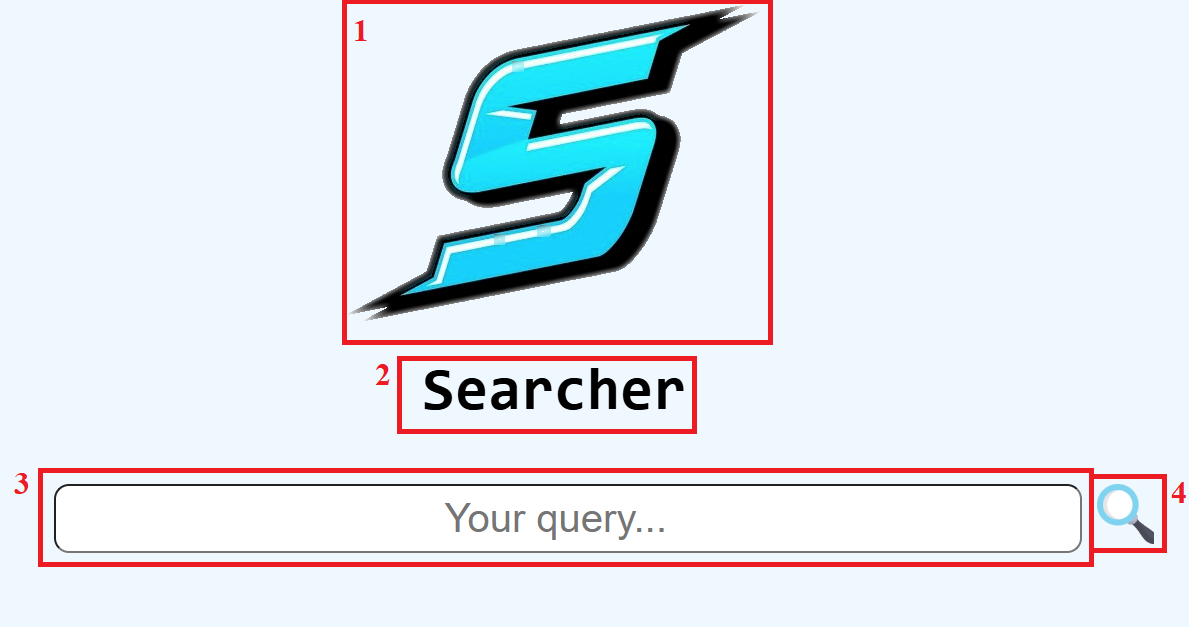
\includegraphics[width=1\linewidth]{web/main.png}}
\caption{Макет интерфейса стартовой страницы}
\label{web/main.png:image}
\end{figure}
Макет содержит следующие элементы:
\begin{enumerate}
\item Поле логотипа поисковика.
\item Поле заголовка поисковой страницы.
\item Поле ввода пользовательского запроса.
\item Кнопка для начала поиска по запросу.
\end{enumerate}

На рисунке 3.16 представлен макет интерфейса страницы отображения результатов поиска.
\begin{figure}[H]
\center{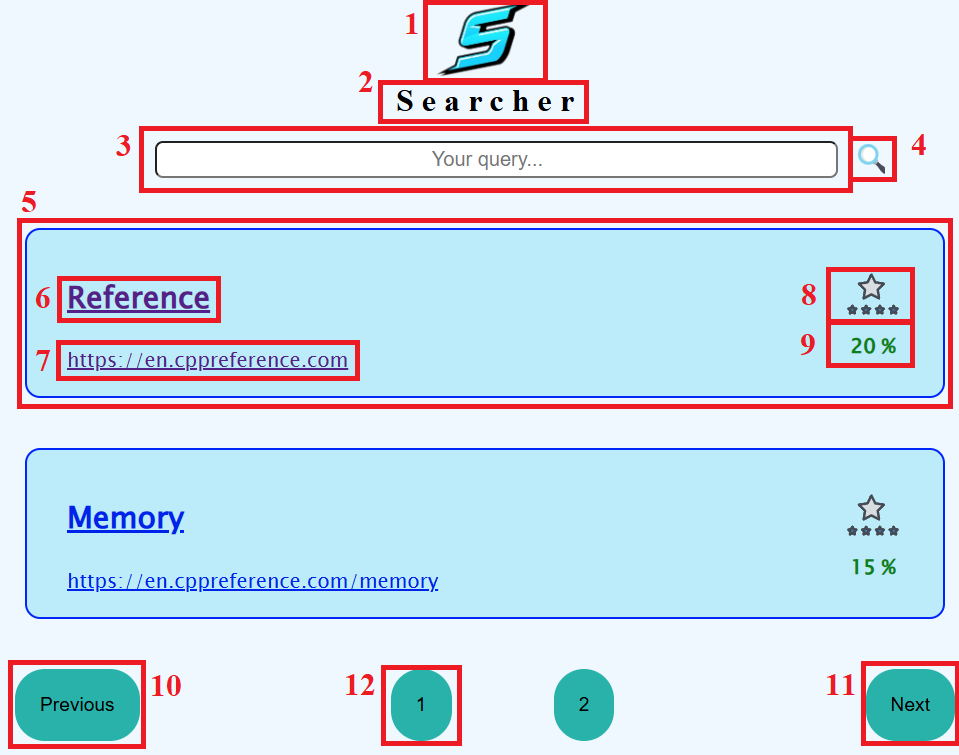
\includegraphics[width=1\linewidth]{web/results.png}}
\caption{Макет интерфейса страницы отображения результатов поиска}
\label{web/results.png:image}
\end{figure}
Макет содержит следующие элементы:
\begin{enumerate}
\item Поле логотипа поисковика.
\item Поле заголовка поисковой страницы.
\item Поле ввода пользовательского запроса.
\item Кнопка для начала поиска по запросу.
\item Элемент отображения одного результата поиска.
\item Поле заголовка ресурса.
\item Поле URL ресурса.
\item Поле иконки релевантности результата.
\item Поле отображения релевантности результата в процентном соотношении.
\item Кнопка перехода на предыдущее множество страниц результатов поиска.
\item Кнопка перехода на конкретную страницу результатов поиска.
\item Кнопка перехода на следующее множество страниц результатов поиска.
\end{enumerate}